% !TEX root = ../../thesis.tex

\section{Numerics}
Proving quantities are conserved is a great way of theoretically verifying our results are correct. However in practicality the reason that numerical analysts are interested in this area of mathematics is to create more precise numerical schemes. We shall now show that normal numerical schemes sometimes provide non-realistic solutions and show how we can produce more realistic results.\\

\noindent
We shall take the standard Euler equations as a simplistic example to show our point. Consider the following Euler equation.
$$ \pd {\vec u} t + ({\vec u} \cdot\nab){\vec u} = 0. $$
We can run a Crank-Nicholson scheme on this. It is well known that Crank-Nicholson is symplectic, that is it preserves the symplectic form. Further, this means that it conserves energy. These schemes can be adapted to conserve other quantities. To motivate these we consider a finite element scheme with a cubed $50\times 50$ grid with order $2$ Lagrange elements. We set an initial condition of,
$$ u_0(x,\, y) = \left( -\cos \left( \frac{\pi x}{2} \right)\sin \left( \frac{\pi x}{2} \right),\, \sin\left( \frac{\pi x}{2} \right)\cos \left( \frac{\pi y}{2} \right) \right), $$
and Neumann boundary conditions. The finite element scheme solves for the spatial steps and we use a Crank-Nicholson for the temporal steps. Hence our scheme is,
$$ \frac{{\vec u}^{n+1} - {\vec u}^n}{\D t} = \frac{1}{2}\left( \left({\vec u}^{n+1} \cdot \nab\right){\vec u}^{n+1} + \left({\vec u}^{n} \cdot \nab\right){\vec u}^{n}\right). $$
We notice that we haven't produced a weak form of the equation. This is due the Euler equations being unstable with weak forms.
This produces the following simulation in Figure \ref{fig:Sim}.

\begin{figure}[!ht]
  \centering
  \begin{subfigure}[b]{0.475\textwidth}
      \centering
      \includegraphics[width=\textwidth]{./img/energy}
      \caption[Network2]%
      {{\small t = 0.25}}
      \label{fig:energy}
  \end{subfigure}
  \hfill
  \begin{subfigure}[b]{0.475\textwidth}
      \centering
      \includegraphics[width=\textwidth]{./img/helicity}
      \caption[]%
      {{\small t = 0.5}}
      \label{fig:helcity}
  \end{subfigure}
  \label{fig:conserv}
\end{figure}

\noindent
We can also consider the conserved quantities. In this system we will consider the total energy and enstrophy,
$$ E = \int_M |\vec u|^2\mu \qquad H = \int_M \vec u \cdot \mathrm{rot} \vec u\mu . $$

\begin{figure*}
    \centering
    \begin{subfigure}[b]{0.475\textwidth}
        \centering
        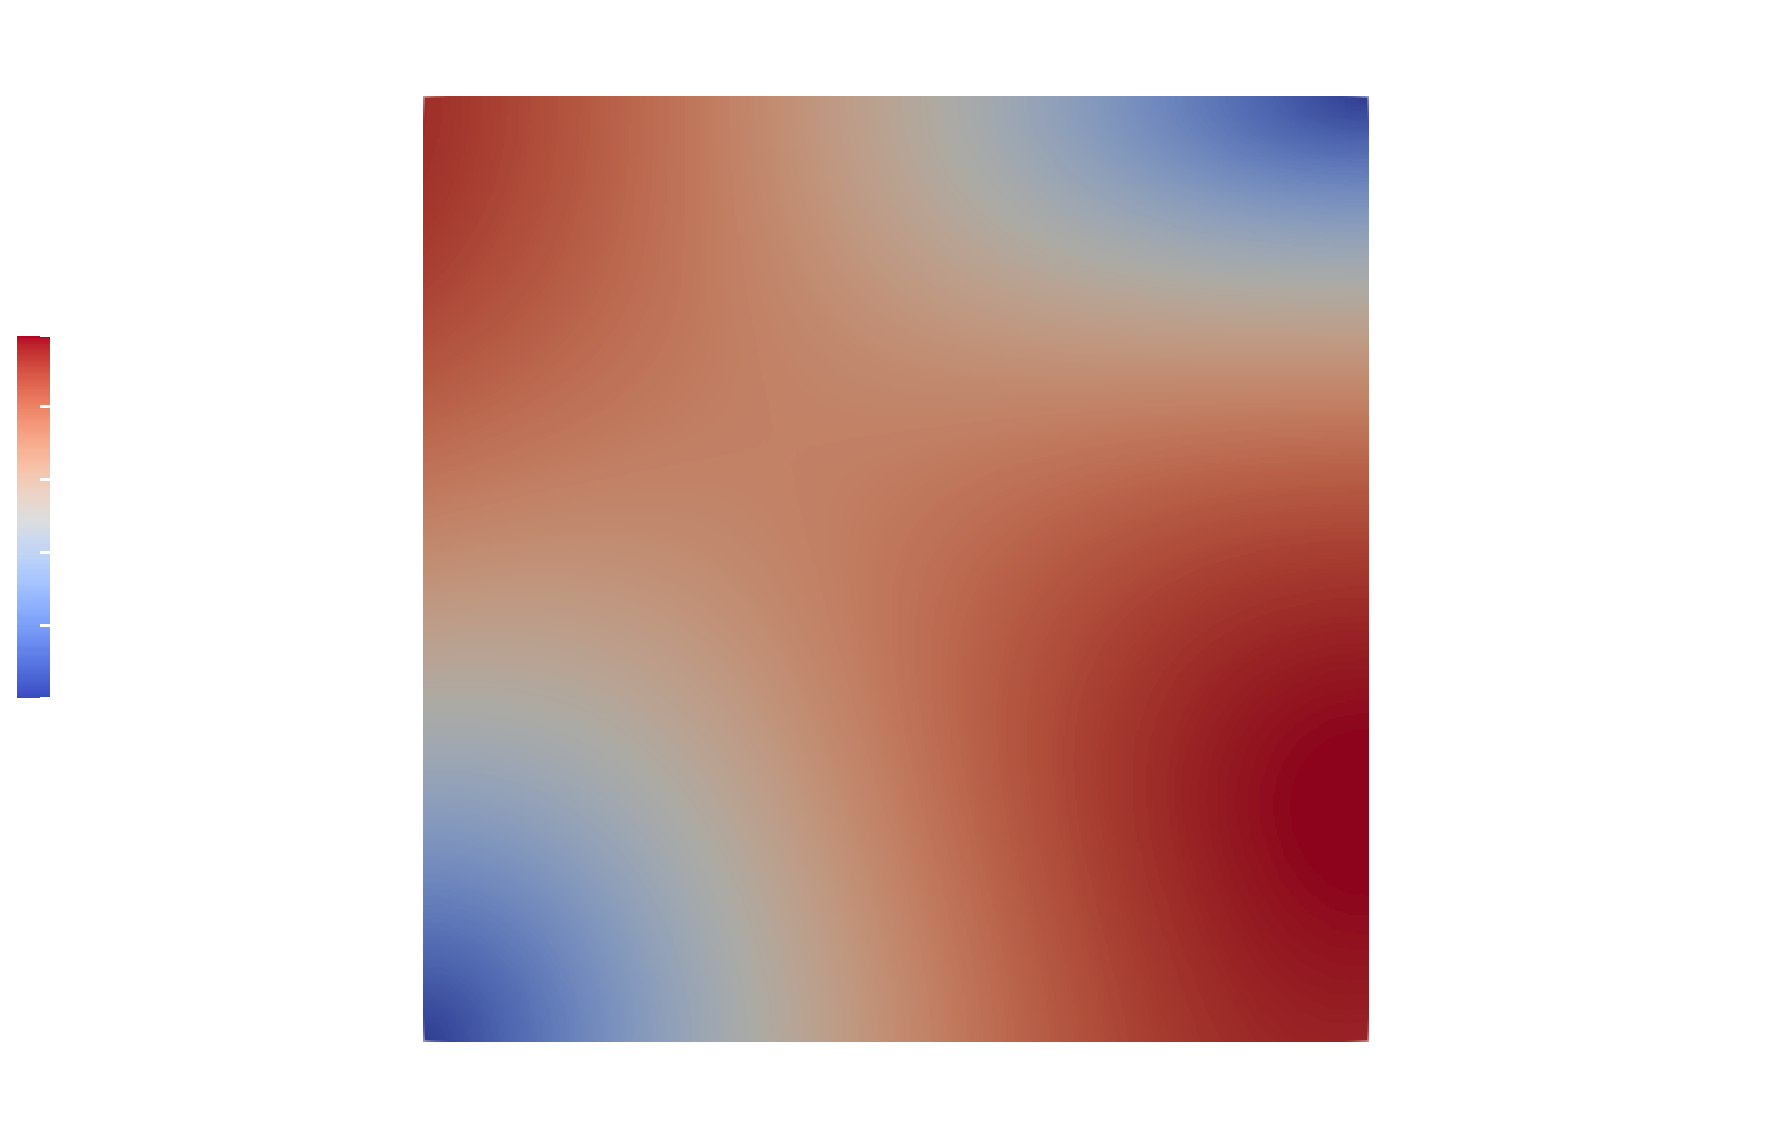
\includegraphics[trim={5cm 0 5cm 0}, clip,width=\textwidth]{./img/25.eps}
        \caption[Network2]%
        {{\small t = 0.25}}
        \label{fig:0.25}
    \end{subfigure}
    \hfill
    \begin{subfigure}[b]{0.475\textwidth}
        \centering
        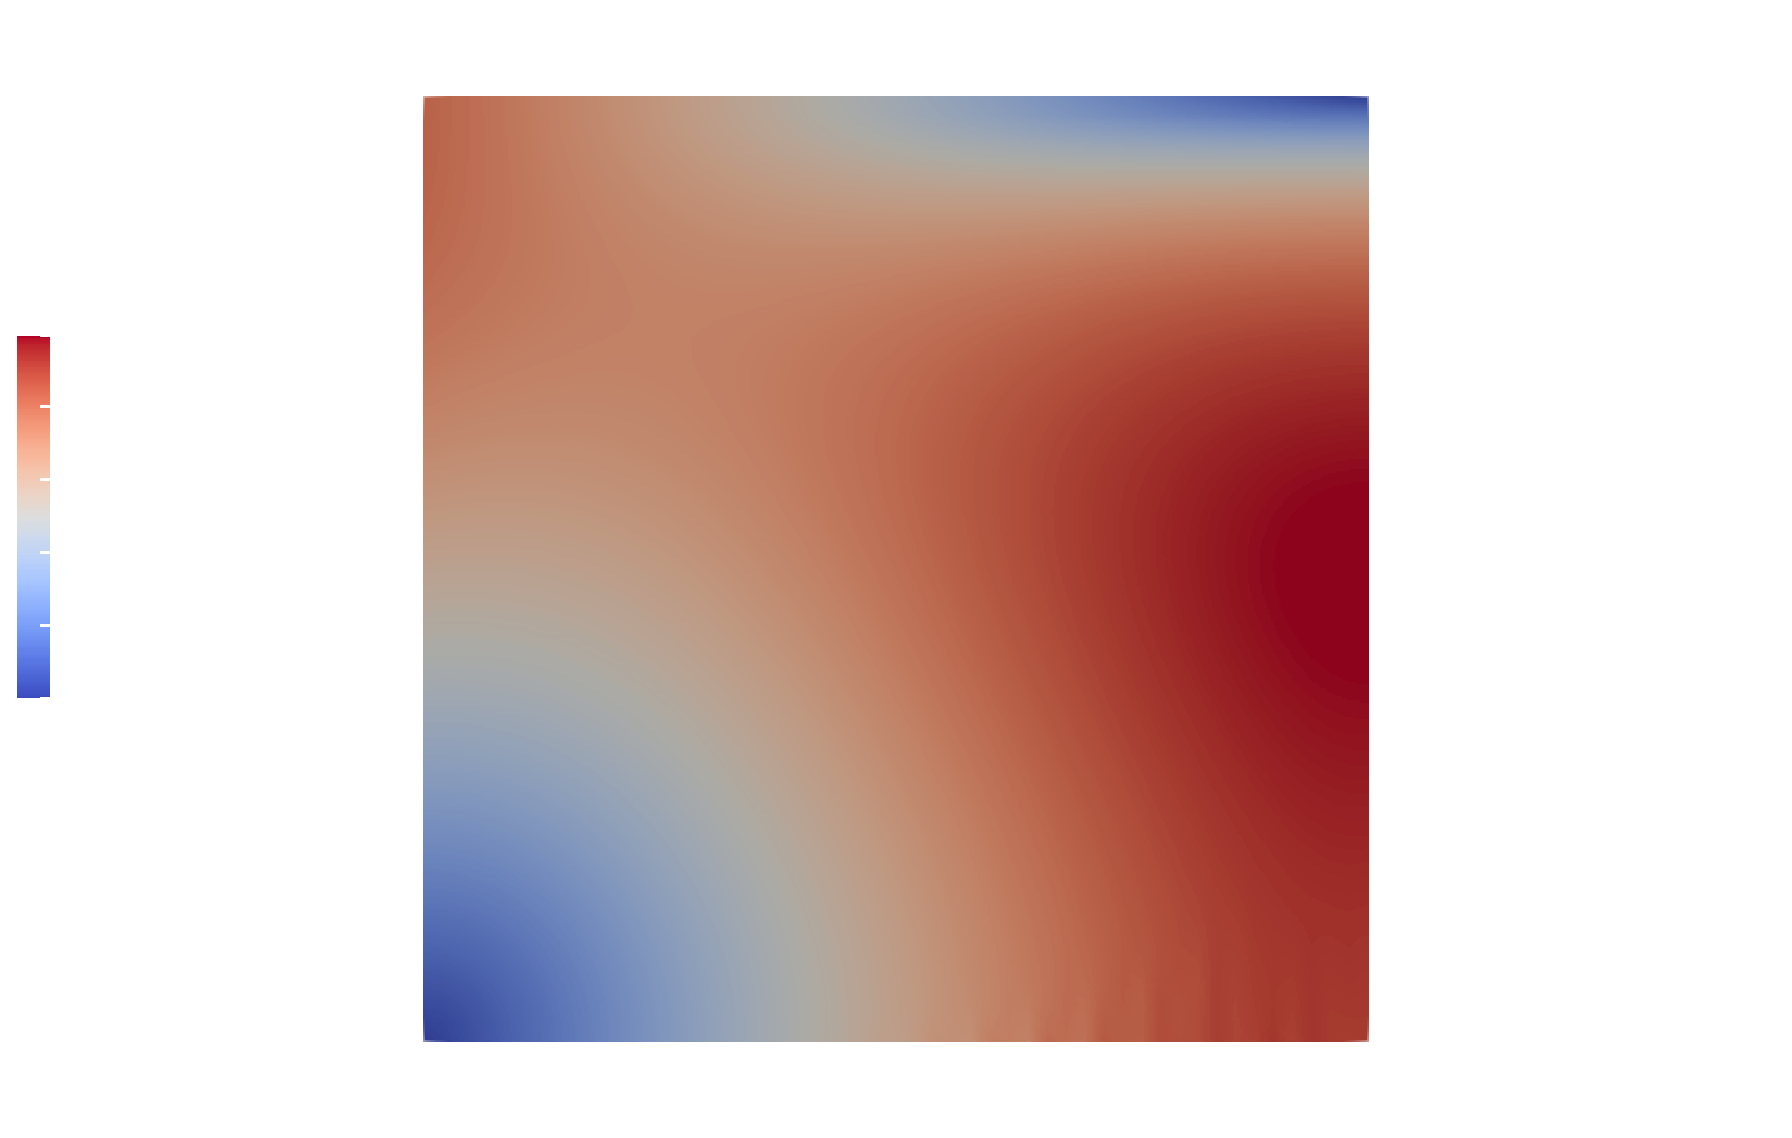
\includegraphics[trim={5cm 0 5cm 0}, clip,width=\textwidth]{./img/50.eps}
        \caption[]%
        {{\small t = 0.5}}
        \label{fig:0.5}
    \end{subfigure}
    \vskip\baselineskip
    \begin{subfigure}[b]{0.475\textwidth}
        \centering
        \includegraphics[trim={5cm 0 5cm 0}, clip,width=\textwidth]{./img/75.eps}
        \caption[]%
        {{\small t = 0.75}}
        \label{fig:0.75}
    \end{subfigure}
    \hfill
    \begin{subfigure}[b]{0.475\textwidth}
        \centering
        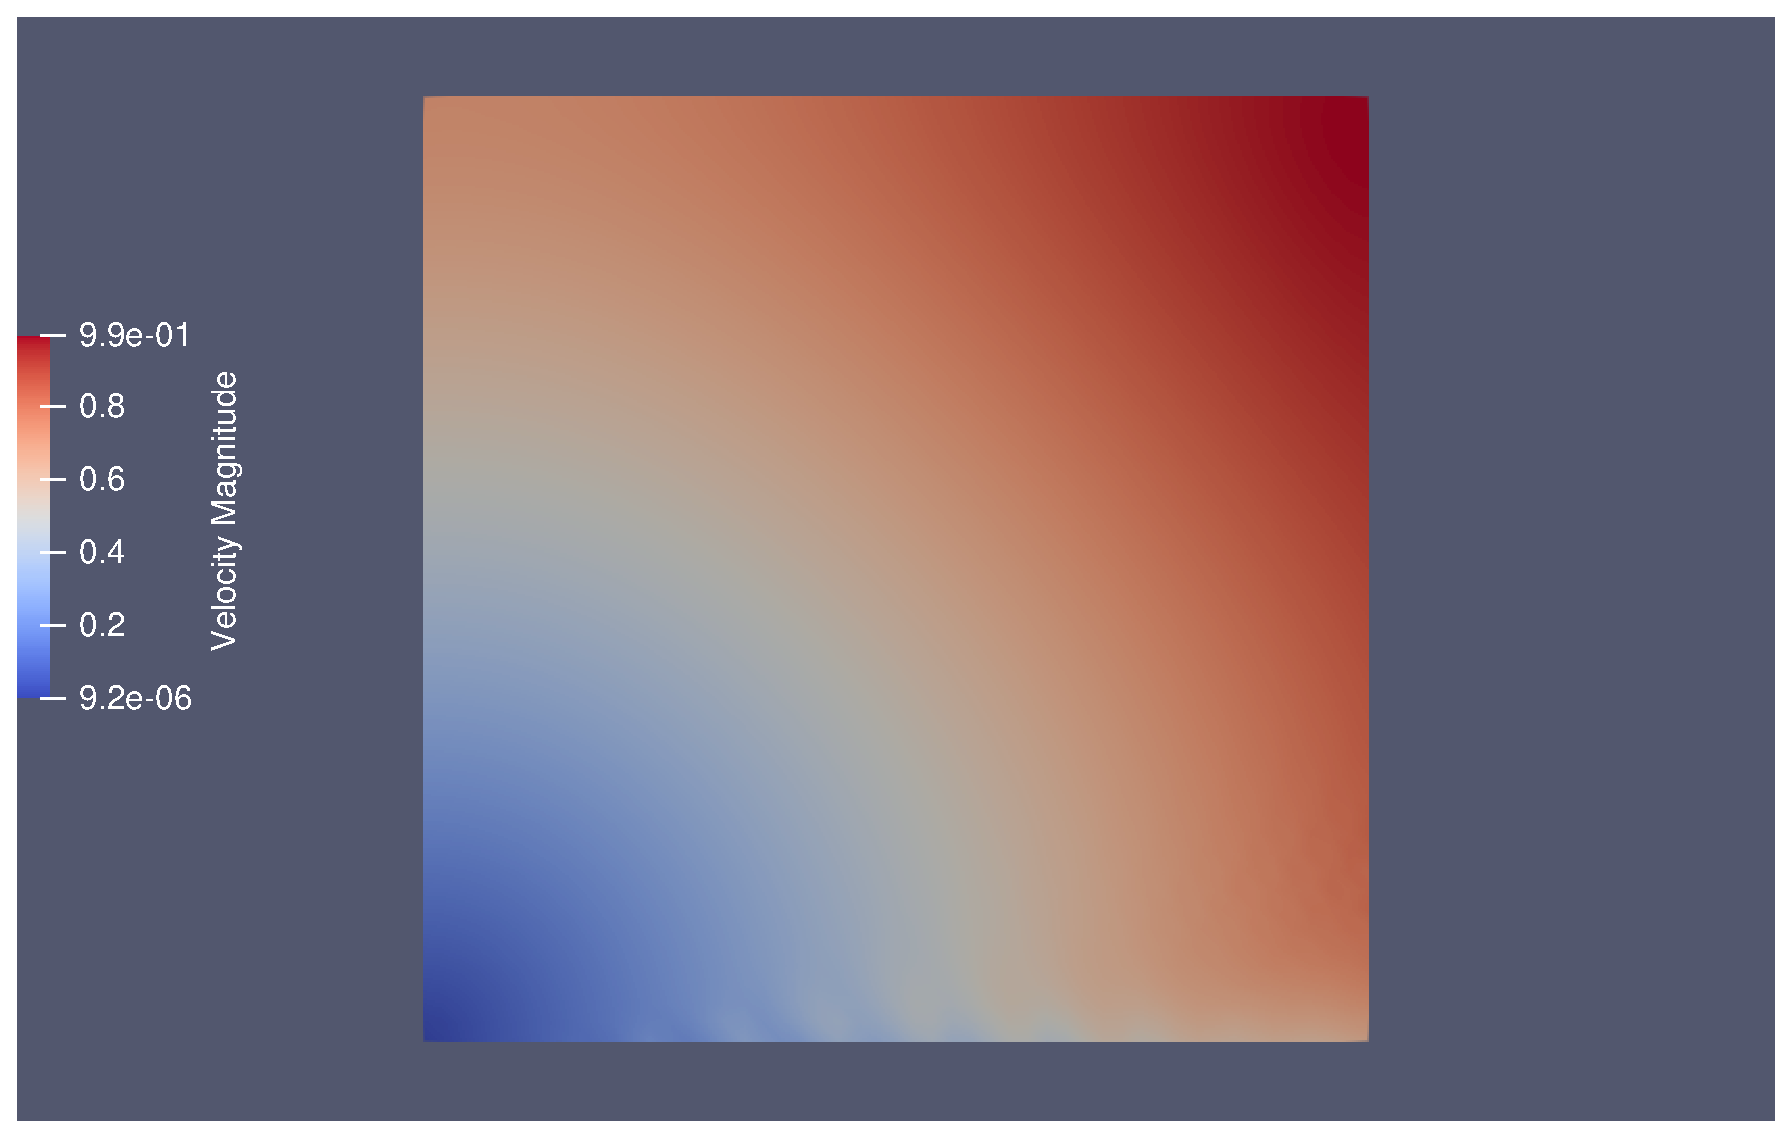
\includegraphics[trim={5cm 0 5cm 0}, clip,width=\textwidth]{./img/100.eps}
        \caption[]%
        {{\small t=1}}
        \label{fig:1}
    \end{subfigure}
    \caption[ Solution to the Euler Equation using a FEM with L_2 elements ]
    {\small Solution to the Euler Equation using a FEM with Lagrange elements}
    \label{fig:Sim}
\end{figure*}
\newpage
\noindent
We notice that the conserved quantities in Figure \ref{fig:conserv}, are unfortunately presenting non-conservation. Due to us using a Crank-Nicholson timestep, which is symplectic, we can say that the error in our scheme comes from our spatial approximation. This is expected as in general finite element schemes are not structure-preserving or symplectic. This leads us to search for a new scheme that allows us to conserve these quantities. We will overview the theory of structure preserving numerical methods and then implement a method. \\

\noindent
The idea is as follows, we can discretise the theory we have presented in this document. Let $F : T^*Q \ti \R \to T^*Q$ be an integrator, where $T^*Q$ is just the tangent space of a phase space, manifold, $Q$ and $\R$ is the space where the time steps $h$ live in. Then we can derive discrete Euler-Lagrange equation from a discrete Lagrangian $L_d : TQ \ti \R \to \R$ and discrete Hamilton's equations from $H_d : T^*Q\to \R$.\\

\noindent
FINISH OFF SOMEHOW?!!?
